\chapter{Frankenbot: System Overview and Capabilities \label{cha:chapter3}}
In this chapter you can find all the details about implementation of a framework utilized to design the bot known as "Frankenbot". Additionally, there is a complete description for a system's architecture, features and abilities of a framework. 
% Lastly, the chapter will be closed by highlighting future goals along with the conclusion.
\\~\\
If you are wondering from where does the name "Frankenbot" came from and why? So firstly, let me remove your confusion. It is derived from the fictional character known as "Frankenstein". It was first introduced in a novel written by Marry Shelley in 1818, Later on after getting hype it was promoted using different media sources like films, T.V. series and also adopted by gaming industry. Furthermore, the most well known edition for its representation was the movie renowned by its original name released in 1931 \cite{frankenstein}. In this movie, Frankenstein was pictured as a haunted scientist who loved to dig the graves of humans and used to create new living being by reassembling their expired body parts \cite{frankensteinmovie}. Likewise, frankenbot is also a composition of different components as explained below in detail.

\section{Why Frankenbot?}
Currently there are many state of the art dialogue frameworks available in the market like Rasa, Plato and IBM Watson. But the question rises why frankenbot and what makes it different from other well known frameworks. There exist following challenges that still need to be addressed.
\\~\\
Firstly, the question raises in mind that, is it possible to design a chatbot that is composed of several small chatbots? Secondly, what if the answer is yes? And one can build a giant chatbot using tiny virtual assistants then how can be the components and modules of a chatbot can be reused? Thirdly, how to make a chatbot independent of technologies used for its development that can cause compatibility issues across different devices? In addition to that, another problem is the re-usability of a dialogue between different chatbots. Furthermore, there is another complication that can not be ignored is the rigidity handling for a chatbot. Which proposes to inject the flexibility to a chatbot so that it can understand the dialogue consisting of multiple topics without displaying any alert message like "You are currently in the middle of current dialogue. Are you sure to abort it?". Lastly, the biggest challenge is to design a chatbot that is capable of staying in to the topic. Which means, it should be able to save the current dialogue state for each user instead of just responding with an answer that matches the user utterance irrespective of the current context in the conversation. 
\\~\\
For above mentioned challenges, there comes the Frankenbot to rescue and addresses them well.

\section{Frankenbot: Approach}
The Frankenbot is a chatbot composed of the parts of multiple chatbots. The design composes modules that work together to form a chatbot as shown in Figure \ref{fig:frankOver}.
\begin{figure}[h]
    \centering
    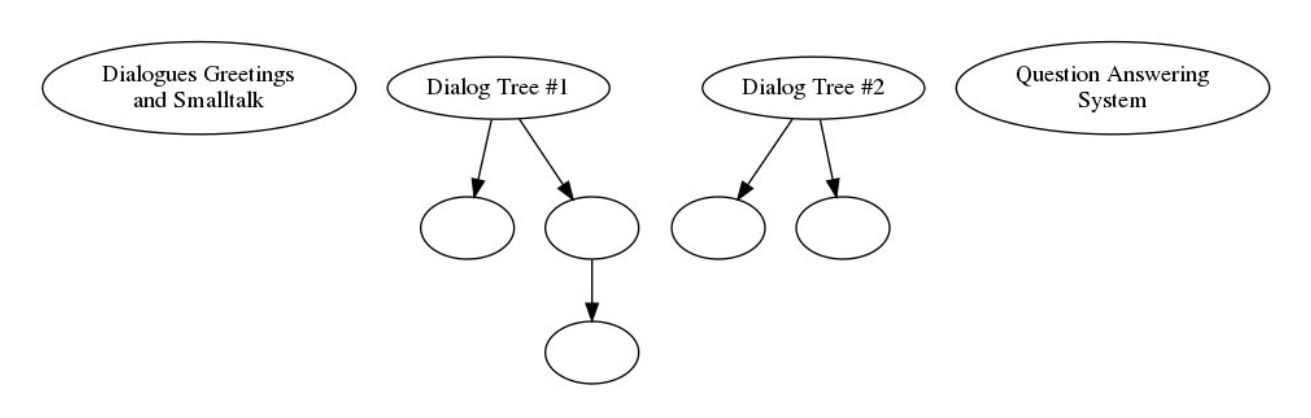
\includegraphics[width=0.9\textwidth]{img/Frankenbot_Overview.PNG}
    \caption{Frankenbot Overview}
    \label{fig:frankOver}
\end{figure}

\subsection{Module}
A module can provide the answer to a user utterance. Therefore it requires an activation function Z that maps the current user utterance and the system state to a real number.
\begin{align*}
 Z: utterance, state \rightarrow R
\end{align*} 
For every user utterance the dialogue manager calls all activation functions and chooses the model with the highest activation function. This module can then generate the answer. The module itself can be anything. It can be a classical intent based system. Other systems are also possible. Some common examples for the modules are as follows:
\begin{itemize}
\item Bag of query/response pairs.
\item Waterfall Dialogue.       
\item Slot-filler Dialogue.
\item Dialogue tree.
\item Question and answering module.
\item Reasoning Module (Knowledge Graphs).
\item Micro domains (MetateM).
\end{itemize}
\\~\\
A module can be more then a dialogue tree. Other systems (question answering, neural systems etc.) can also fit in this framework, as long as they implement an activation function.
\\~\\
The classic slot-filler/single dialogue tree based architecture is a basic possible module of the Frankenbot. Therefore the Frankenbot is at least as powerful as the slot-filler.

\subsection{Modular Architecture}
There are some benefits for using modular architecture. Just for example, consider a dialogue with two dialogue sub-trees as shown in Figure \ref{fig:modArch}. In a traditional system we need to model:
\begin{itemize}
\item The transitions from the root node to the sub-tree.
\item The transitions inside each sub-tree.       
\item The transitions from each node to the root node(dashed lines: “I want to cancel this dialogue”).
\item To enable transitions between the sub-trees they would need to be modelled explicitly. In the example this is omitted due to the complexity of the graph. Also it is not possible to go back and continue from the previous sub-tree.
\end{itemize}

\begin{figure}[!h]
    \centering
    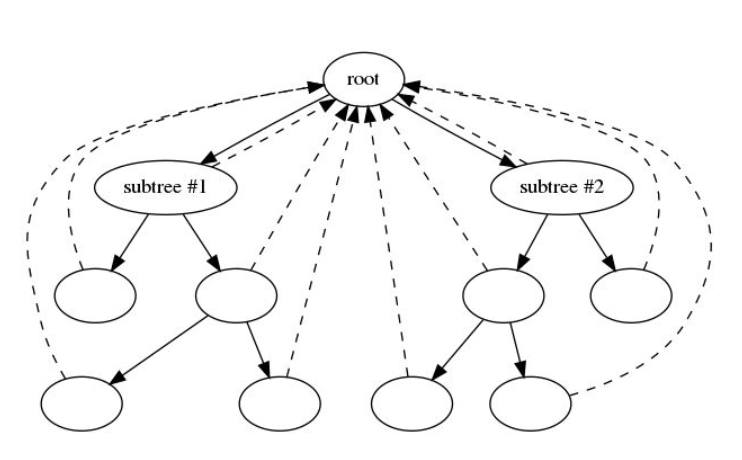
\includegraphics[width=0.9\textwidth]{img/Modular_Architecture.PNG}
    \caption{Dialogue with two sub-trees without Modular Architecture}
    \label{fig:modArch}
\end{figure}

\subsubsection*{Modular Architecture's Characteristics}
By using this architecture many features can be unlocked. Reusability and performance can also be enhanced as mentioned below:

\paragraph*{Simpler but robust dialogue trees\label{par:simplerTree}}
The same dialogue as mentioned above but with the Frankenbot's framework modular architecture is shown in Figure \ref{fig:modArch2}. As you can notice the dialogue tree is less complicated and more powerful.
\begin{itemize}
\item Jump back to root node is not necessary.
\item Switching between trees is possible without explicit modelling.       
\item Going back after switching is possible without explicit modeling.
\end{itemize}

\begin{figure}[!h]
    \centering
    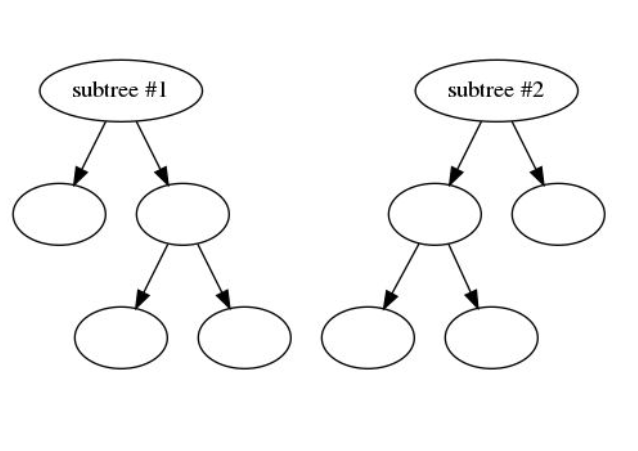
\includegraphics[width=0.9\textwidth]{img/Modular_Architecture_2.PNG}
    \caption{Dialogue with two sub-trees using Modular Architecture}
    \label{fig:modArch2}
\end{figure}

\paragraph*{Unification of Smaller Chatbots}
In this framework, all modules remain independent of each other. They are not tied together. Using this architecture the complexity of larger chatbots can be declined by dividing them in to smaller liberated bots. In other words, we can approach the complexity of larger chatbots using divide and conquer rule. This modular architecture provides a better framework for giant bots to grow. It also provides more customization options to a bot as one can easily add and remove any module from any bot at any time without caring for its dependencies.

\paragraph*{Modules Reusability}
Modules can be reused within a same chatbot or different chatbots:

\begin{itemize}
\item \textbf{Reusability within a Chatbot:} Modules can be reused with in a chatbot. Just consider an example as shown in the Figure \ref{fig:modReus2}. 
\\~\\
Imagine a chatbot from the smartphone support domain. Two dialogues require how to find out the model of the smartphone. The smartphone model will be stored as environment variable. Transitions with a diamond tail are only possible when this environment variable is set. The transition with the dashed line does not leave the current node. It only activates the node in the next tree.
\begin{figure}[!h]
    \centering
    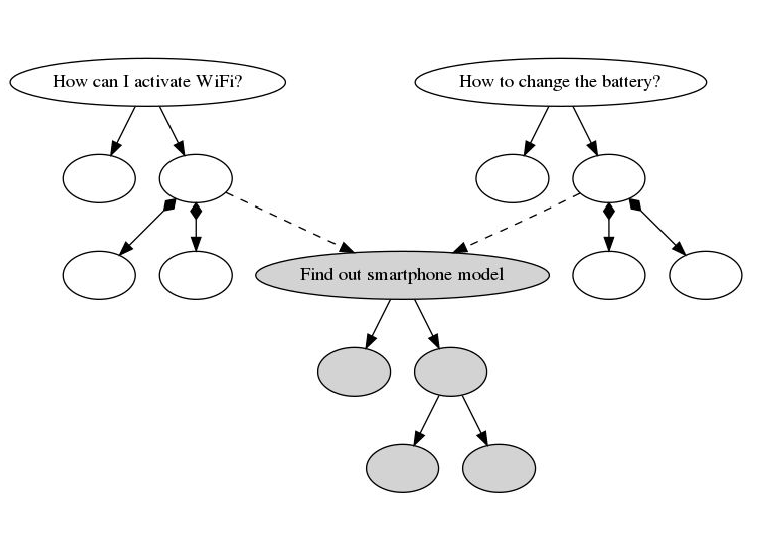
\includegraphics[width=0.9\textwidth]{img/Module_Reusability_2.PNG}
    \caption{Module reusability within a chatbot}
    \label{fig:modReus2}
\end{figure} 
\\~\\
The same dialogue graph with a traditional dialogue tree has shown in the Figure \ref{fig:modReus3} which has several restrictions and disadvantages. The module should be defined twice, more explicit relations needed to go back from one state to another and the dialogue trees are more complicated. Also the number of nodes and transitions will be higher as considered to Frankenbot's Architecture resulting to higher processing as shown in the Table \ref{tab:tradVsFran}.
\begin{figure}[!h]
    \centering
    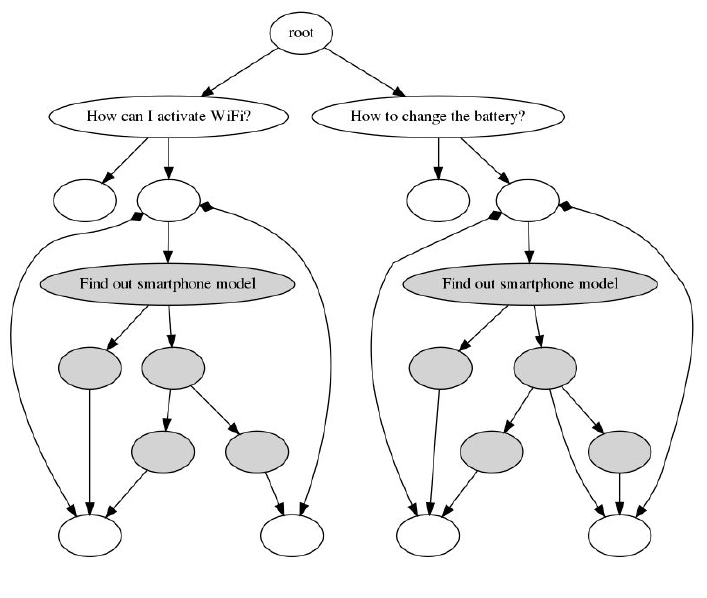
\includegraphics[width=0.9\textwidth]{img/Module_Reusability_3.PNG}
    \caption{Module reusability within a chatbot}
    \label{fig:modReus3}
\end{figure}

\begin{table}[!h]
    \centering
   \begin{tabular}{ |c|c|c|c| } 
        \hline
         & No. of Nodes & No. of Transitions \\
        \hline
        \row{Traditional} & 21 & 26 \\ 
        \row{Frankenbot} & 15 & 14 \\ 
        \hline
    \end{tabular}
    \caption{Traditional vs. Frankenbot in terms of nodes and transitions}
    \label{tab:tradVsFran}
\end{table}

\item \textbf{Reusability among different Chatbots:} Reusability can be enhanced by using modular architecture. Multiple chatbots can share common modules. The module needs to be defined only once. Changes in the module will automatically be integrated in all chatbots. Figure \ref{fig:modReus} shows visuals for better understanding of it. 
\begin{figure}[!h]
    \centering
    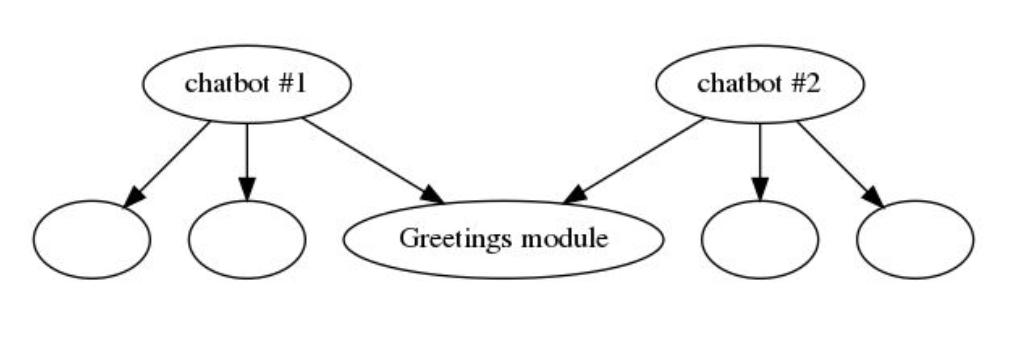
\includegraphics[width=0.9\textwidth]{img/Module_Reusability.PNG}
    \caption{Module reusability between different chatbots}
    \label{fig:modReus}
\end{figure}       
\end{itemize} 

\paragraph*{Sense for Staying in the Topic}
The dialogue manager chooses the module with the highest activation function. But we can also add a term to stay in the topic: 
\begin{align*}
 Activation(module) = Z(utterance, state) + History(module)
\end{align*} 
Z is the activation function. History(module) is a term that gets bigger if the module has been active before. Therefore the module that was used before has a higher probability of being chosen which refers to the chatbot staying in the topic characteristic.

\section{Frankenbot: System Architecture}
The architecture consists of a server and server-side web API. The user communicates with the help of a browser, and sends request to a server having the framework deployed on it. User sends a request from the browser using web API which communicates with a server. Furthermore, server contains deployed Frankenbot's framework built using Python 3. Web server loads a data for a chatbot from json file for now but will be integrated with some database in future. Whereas, frontend for user's interaction has built simply using javascript, html and css. Web API has been built using python library known as Flask \cite{flask}. The architecture has shown in the Figure \ref{fig:sysArch}.

\begin{figure}[!h]
    \centering
    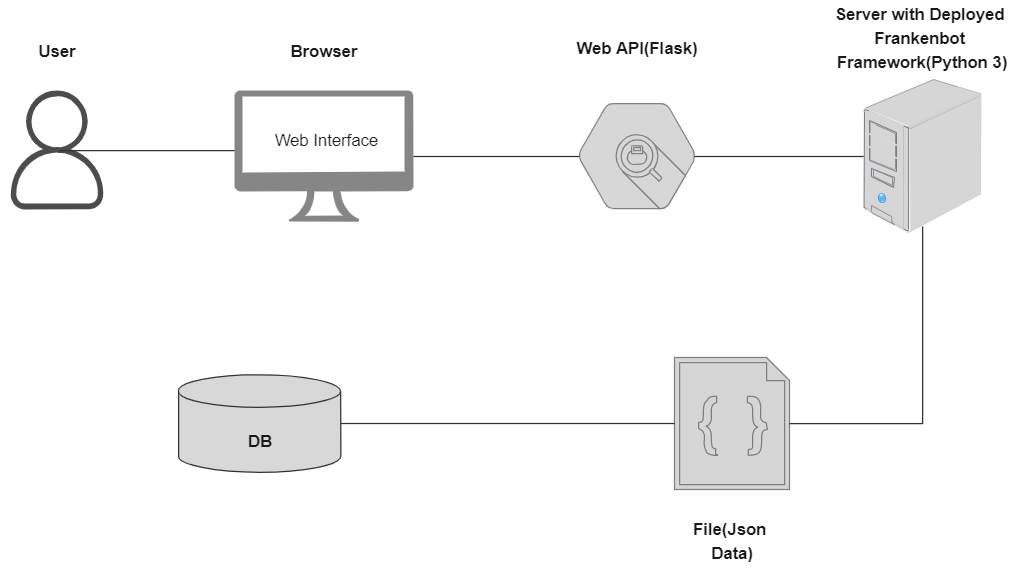
\includegraphics[width=0.9\textwidth]{img/System_Architecture.PNG}
    \caption{Frankenbot's System Architecture}
    \label{fig:sysArch}
\end{figure} 
\\~\\
As it is clear from the Figure \ref{fig:sysArch} that the communication between client and the server is possible only via web API composed of simple get request. In addition to that when you dig deep in to the framework, it is composed of several different components. For detailed discussion refer to the next section.

\subsection{RASA Framework for NLU}
RASA is an open source renowned conversational artificial intelligence framework for designing contextual virtual agents. It is a machine learning framework designed to communicate by means of automated text and voice-based techniques. \cite{rasa}
\\~\\
For making it work, following steps must be taken in to account:
\begin{enumerate}
    \item Provide training data \cite{rasatrainingdata}.
    \item Provide configuration file with pipelines for training \cite{rasapipeline}.
    \item Provide directory's path to save trained models.
    \item Generate rasa interpreter by loading it from the trained models directory.
\end{enumerate}
For utilizing it in a Frankenbot, necessary steps have been mentioned below under the heading of Configurations.
% \ref{par:config} in Frankenbot's Framework.
 
\subsubsection*{Training for RASA}
It has been used for natural language understanding in Frankenbot. It needs to get trained first in order to produce some useful results and for that purpose one needs to provide it with the training data. It can be provided using different formats as mentioned on its website \cite{rasatrainingdata}. For Frankenbot, json format has been adopted but it can be changed without any issue based upon the developer preference. This format consists of a top-level object called rasa\_nlu\_data, with the keys common\_examples, entity\_synonyms and regex\_features. The most important one out of these all is common\_examples.

\begin{lstlisting}[language=json,firstnumber=1]
{
    "rasa_nlu_data": {
        "common_examples": [],
        "regex_features" : [],
        "lookup_tables"  : [],
        "entity_synonyms": []
    }
}
\end{lstlisting}
 Moreover, common\_examples is a list of objects with the keys text, intent and entities. Whereas, entities can be an empty list or the objects list with the keys start, end, value and entity.
 
 \begin{lstlisting}[language=json,firstnumber=1]
{
    "text": "...",
    "intent": "#...",
    "entities": [
            {
                "start": ...,
                "end": ...,
                "value": "...",
                "entity": "@..."
            },
            ...
    ]
}
\end{lstlisting}

\subsection{Frankenbot's Framework}
This framework is composed of various components. Each of which is responsible for performing a specific task. It is divided majorly in to two divisions. First one is the web server(backend), which is responsible for creation of the whole chatbot and producing desired responses for a user. While the other one is client(frontend) also known as user interface to interact with a chatbot. Both of these are explicitly explained below in detail.
\\~\\
The detailed diagram for Frankenbot's Framework Architecture has been portrayed in the Figure \ref{fig:frankArch}. All the components have been discussed in detail afterwards.

\begin{figure}[!h]
    \centering
    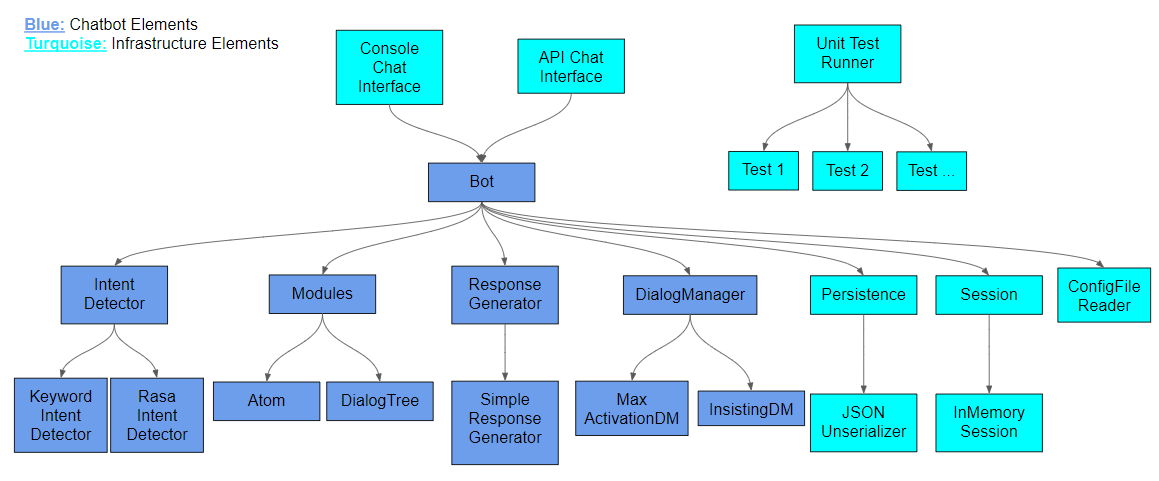
\includegraphics[width=0.9\textwidth]{img/Frankenbot_Architecture.PNG}
    \caption{Frankenbot's Framework Architecture}
    \label{fig:frankArch}
\end{figure} 

\subsubsection*{Client}
It is implemented using simple JavaScript, Html and CSS. The template can be found under \cite{userinterface}. It is a simple user interface for a chat which allows a user to type a message and send it to the server by making simple get request by means of the web API. 
\\~\\
Furthermore, it is also responsible for storing user's session id to a storage on a browser. For that purpose browser's "localStorage" \cite{localstorage} is used. If user is connected to the first time to the server then it requests with an empty session id and user utterance to the server. And as a response chatbot sends a welcome message and assigns an id to a user. Which is saved in the browsers local storage for every user. Whenever there comes a new request from this user to a server, the session id is being sent along with a user utterance to a server. In return, server responds back with a suitable response according to the user utterance which is being displayed next to the last user utterance. The response from the server is in a form of a json object which is being parsed to extract the chatbot's reply and displayed for a user. The important point to take in to account is that the user id will be stored until the page is not reloaded or closed. If you want to restart your session and get away with all your previous chat, then you can simply refresh the web page and it will make a new instance of the chatbot. But for future, server will have the record of all dialogues happened in a past stored in a database. 
\\~\\
For better understanding graphical representation for an interface is shown in the Figure \ref{fig:userInter}.

\begin{figure}[!h]
    \centering
    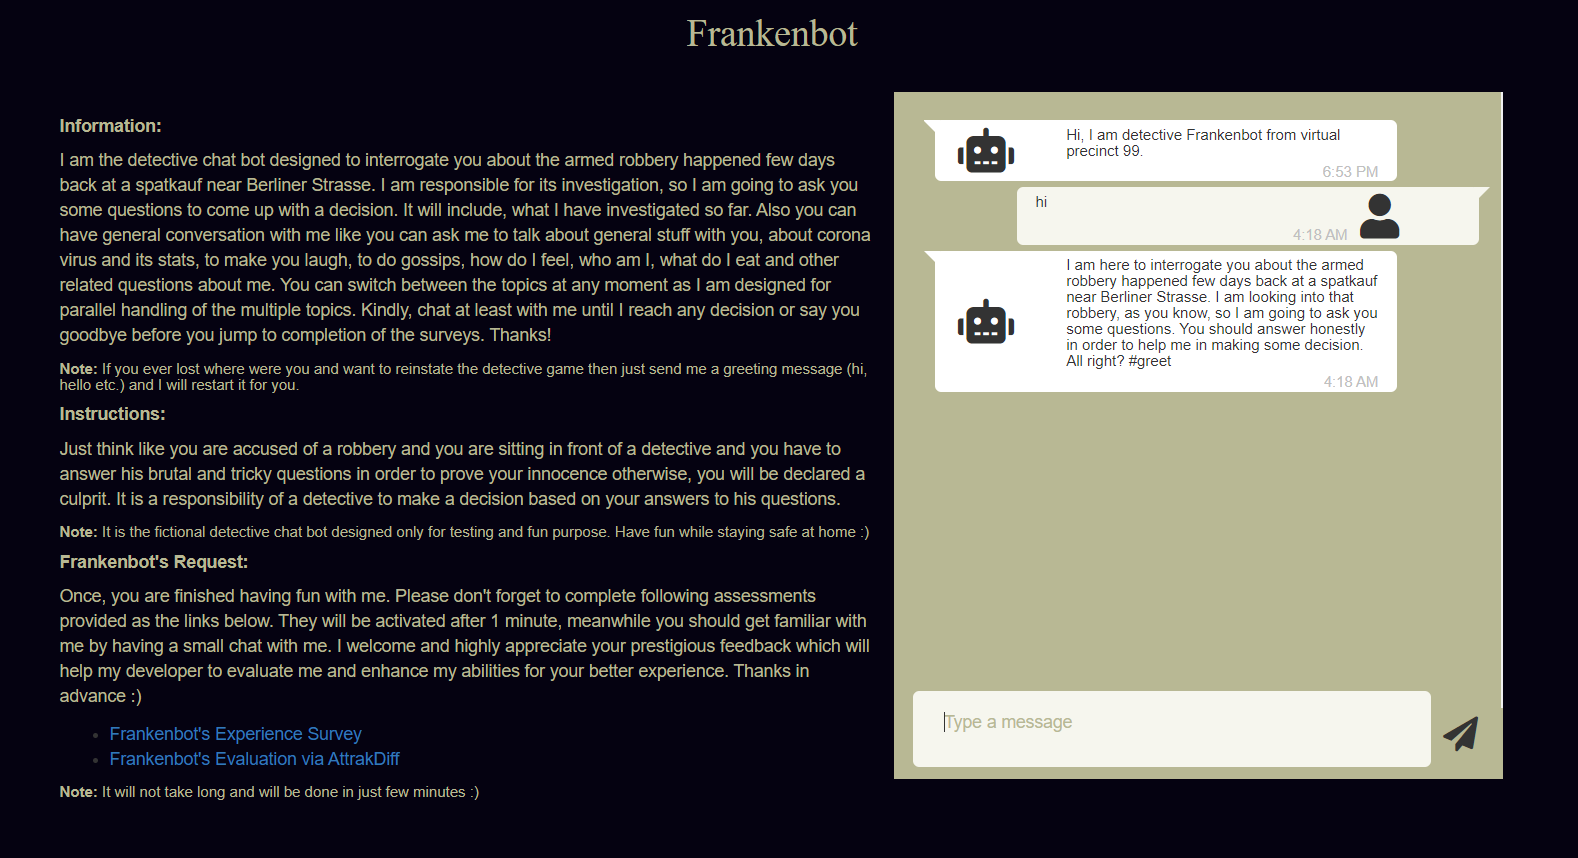
\includegraphics[width=0.9\textwidth]{img/User_Interface.PNG}
    \caption{Frankenbot's User Interface(Client)}
    \label{fig:userInter}
\end{figure}
\\~\\
As you can see in the Figure \ref{fig:userInter} that  on the left side of the screen, the important information and instructions for new user has been displayed. Whilst, on its right, there exists a chat box showing the first most message as a welcome message for new user. After that the chat between the user and a bot initiated. The user can type a message in the bottom most text box and press send button or enter button from keyboard. User's message will be displayed on left side of screen while response will be shown on right side of screen's display and vice-versa according to your view point.

\subsubsection*{Web Server}
Web server itself is a composite of multiple classes performing specific tasks and connected to a client using web API. It is written in Python version 3. Abstractly, it is responsible for performing all tasks required to make a chatbot functioning. Firstly it receives user utterance as a parameter and initializes a chatbot from data provided as a source file of json format. After initializing a chatbot, it undergoes various actions for an user utterance in order to generate a response.

\paragraph*{Infrastructure Elements}

\subparagraph*{Web API}
It is implemented using python library known as Flask. It is responsible for making a connection between user and a server. It makes a user to communicate with a server. Whenever, there comes a new request from the client, firstly it passes from the function implemented for its handling.
\\~\\
Important tasks performed by the web API are:
\begin{enumerate}
    \item Receiving the user utterance and session id as a parameter from the get request made by the client.
    \item Checking whether the session id already exists or its a new user. If it happens to be a new user then there will be the empty user utterance and user session id received as a parameter from the client's get request. It will initialize a chatbot using the data provided in the json file (discussed in detail below). Afterwards, it assigns a new user session id and sends it along with a welcome message as a response to a client.
    \item If session already exists, then it check for the current dialogue state for an active user. And instead of initializing a new chatbot, the chatbot with the last stored state is being traversed with new user utterance in order to get an appropriate response. And before responding back to the client the current state gets updated again and stored for the current user.
     \item The response is being sent as a json object.
\end{enumerate} 

\subparagraph*{Persistence}
Persistence includes the Json Unseralizer. It takes the json file as an input and parses it for generating an initial chatbot.
\\~\\
The json file contains data as a json dictionary object which includes the name of a bot, welcome message, fallback message in case of no response and a dialogue manager. Inside a dialogue manager there exists a list of modules consisting of several modules having unique module ids. Additionally, each module contains a dialogue tree having a list of tree nodes. Whereas, each tree node includes a unique node id, information about its parent node, name of an intent to which it belongs and respective response generator. Which furthermore includes mode for the responses that can be sequential or random and a list of responses. And all of the above mentioned elements are uniquely identified using a key "type". For better understanding, just have a look on a json sample shown below:
\\~\\
\begin{lstlisting}[language=json, firstnumber=1]
{
  "type": "bot",
  "name": "...",
  "welcome_message": "Hi, ...",
  "fallback_message": "any desired message for bot's failure.",
  "dialog_manager": {
    "type": "max_activation_dialog_manager",
    "modules": [
        {
        "type": "dialog_tree",
        "module_id": "module1 or any id",
        "dialog_tree": [
          {
            "type": "tree_node",
            "node_id": any integer e.g 1,
            "parent_node": null for making root or any node id  to assign it a parent,
            "intent_name": "#...",
            "response_generator": {
              "type": "simple_response_generator",
              "mode": "sequential or random",
              "responses": [
                ...,
                ...
              ]
            }
          },
          ... ,
        ]
      },
      ... ,
    ]
  }
}
\end{lstlisting}

\\~\\
A bot is generated recursively on the basis of unique type key. The json data has been iterated and checks for the type of each element recurrently. And by taking that type of an element in to account, it returns the object for different respective classes. Let suppose the json object contains types in a following sequence:
\begin{enumerate}
    \item bot; recall the same function with a json for a dialogue manager returns a class Bot's object afterwards.
    \item max-activation-dialogue-manager; recall the same function with a json for each module in a list of modules and returns a class MaxActivationDialogueTreeManager's object afterwards.
    \item dialogue-tree; recall the same function with a json for a dialogue tree and returns a tree consisting of tree nodes afterwards.
     \item tree-node; recall the same function with a json for each element of a list dialogue tree and returns a class Atom's object afterwards.
     \item simple-response-generator; recall the same function with a json for a response generator and returns a class SimpleResponseGenerator's object afterwards.
\end{enumerate} 
\\~\\ 
Now the function initiated from the first step mentioned above, but starts returning from the last step. And each returned object has been passed as a parameter to the constructor of upper level class object. So finally the class Bot object should contain the class MaxActivationDialogueManager's object as an attribute and that is how the chatbot will be generated recursively.
\\~\\
Also, there is a convention used to represent the intents, entities and context variables. It has been taken from the state of the art chatbot IBM Watson as intent is denoted by prefix "\#", entity is denoted by "@" and "\$" symbol is used to denote a context variable. Same convention has been used in Frankenbot as shown in the Table \ref{tab:repIntEntCont}.

\begin{table}[!h]
    \centering
   \begin{tabular}{ |c|c|c|c| } 
        \hline
         & Key & Value \\
        \hline
        \row{Intent} & {\#intent\_name} & {intent\_value} \\ 
        \row{Entity} & {@entity\_name} & {entity\_value} \\
        \row{Context Var.} & {\$context\_var\_name} & {context\_var\_value} \\
        \hline
    \end{tabular}
    \caption{Representation for an Intent, Entity and Context Variable}
    \label{tab:repIntEntCont}
\end{table}


\subparagraph*{Session}
It is responsible for session handling. It is subjected to establish "InMemorySession" which is meant to store session id in a list of session variables, context variables and sequential response counter for each user. For each user there exists a different chatbot's state. 
\\~\\
Whenever there comes a new user, the new dictionary object has been declared to store session id for a user along with its bot's state, active module id and active node for each module. In addition to that the last user utterance also gets stored for generating the last bot's message to user if chat window has been refreshed or reopened in a new tab of browser by a user(can be implemented in future). And then that dictionary object gets appended to a list of session variables. Which means there exists a separate object for each user in a list. It gets updated on every request from the client.
\\~\\
Another element present to save the context of a dialogue for each user is known as context variables. It is a dictionary having user session id as a key, and each key represents a key value pair for entities appeared in a dialogue. Each entity name appeared in a dialogue has been saved as \$EntitytName as a key and a value of entity as its value. Its value gets updated every time if same entity has been triggered or new entity has been discovered in a dialogue from same user. These context variables are used to understand the context of a dialogue and update the entity value in a response if it is intended.
\\~\\
Another important attribute available is response sequential counter. Its main task is to keep track of all intent's response counter for each user if its mode has been set to sequential. It means if an intent contains multiple responses and bot has to produce response for it based on the user utterance then each time next response should be produced for a user. It is intended to give more realistic impression to a user and human like interaction behaviour to a dialogue.

\subparagraph*{Configurations \label{par:config}}
In order to make chatbot work it is really important to provide it with proper configurations. Frankenbot needs three following directories in order to function:
\begin{enumerate}
    \item bot directory; It should be provided with the bot's directory name as a command line parameter while running the project. For example, the running command in my case is "python app.py detective". In this command "detective" is a name of directory which should contain json file for initializing a bot. And it should be named as "frankenbot.json" (see Appendix \ref{appen:frankJson} to have a look on actual json data used for structuring of the Frankenbot). 
    \item Furthermore, the bot directory must contain training data directory named as "rasa". Firstly, this sub-directory must contain a configuration file named as "config\_spacy.yaml" defining pipelines required for Rasa NLU Training\cite{rasapipeline} (see Appendix \ref{appen:rasaConf} to have a look on actual pipelines used). Secondly, json files must be available with a training data for each module in "frankenbot.json". And the names for those training files should be same as module id assigned to a module for which it contains training data. For example, "frankenbot.json" contains two modules and ids assigned to them are detective\_tree and general\_tree. So, the training files should be named as "detective\_tree.json" and "general\_tree.json" (see Appendix \ref{appen:trainDF} to have a look on actual json training data used for both training of modules in the Frankenbot).
    \item Lastly, the model directory is required to store the rasa models produced after the model gets trained for each module. It can be any directory but one has to provide appropriate path to it.
\end{enumerate} 

\paragraph*{Chatbot Elements}

\subparagraph*{Bot}
Once the initial bot is generated, it is the very first element that has been instantiated. Originally it contains the complete definition for a chatbot. Which includes the attributes such as chatbot's name, welcome message, fallback message and most importantly dialogue tree manager(discussed below in next heading).
\\~\\
Whenever, a request from a client has been made it firstly gets processed by this component. As it receives the user utterance, active tree nodes for each module for a particular user and session information as a parameter. These parameters are further passed to its dialogue tree manager in order to find module with highest intent's activation value, detected intent, intent's activation value, detected entities, entities activation values, active tree node, active module id and json output object. This json object has been returned to a client containing all important information and respective response.
\\~\\
Before returning the response as a json object, it is also responsible for performing some major tasks. Firstly, it checks for detected entities received after the processing of its dialogue tree manager. If there exist any detected entity then entity(s) in the context variables for a particular user gets added or updated depending upon the current state of a bot.
\\~\\
In addition to that, it also checks for the detected intent's activation value for a user utterance. As, Rasa Natural Language Understanding has been used to detect the intent and there are the chances of getting false result with very low activation value. So it checks for it, and responds only if its value lies above some threshold. The range of activation value lies between 0 and 1. If the value is below the threshold then it check for the last active node for a user whether it exists or not. If it doesn't exist then, it means user started chat with some meaningless utterance as an input for a bot. So, the chatbot should respond using node with intent anything\_else if it exists in a module with highest activation obtained from rasa nlu's result. Secondly, if there exists some chatbot's active state for a user, then it checks for last active module for a user and also checks for a node with an intent name anything\_else in its children. If it is available then response has been generated using it. Otherwise, it simply responds with a fallback message.
\\~\\
Alternatively, if it is above the threshold then the highest module received from its dialogue tree manager has been used to generate an appropriate response(explained ahead). Complete flow can be observed in the following Figure \ref{fig:flowBot}.

\begin{figure}[!h]
    \centering
    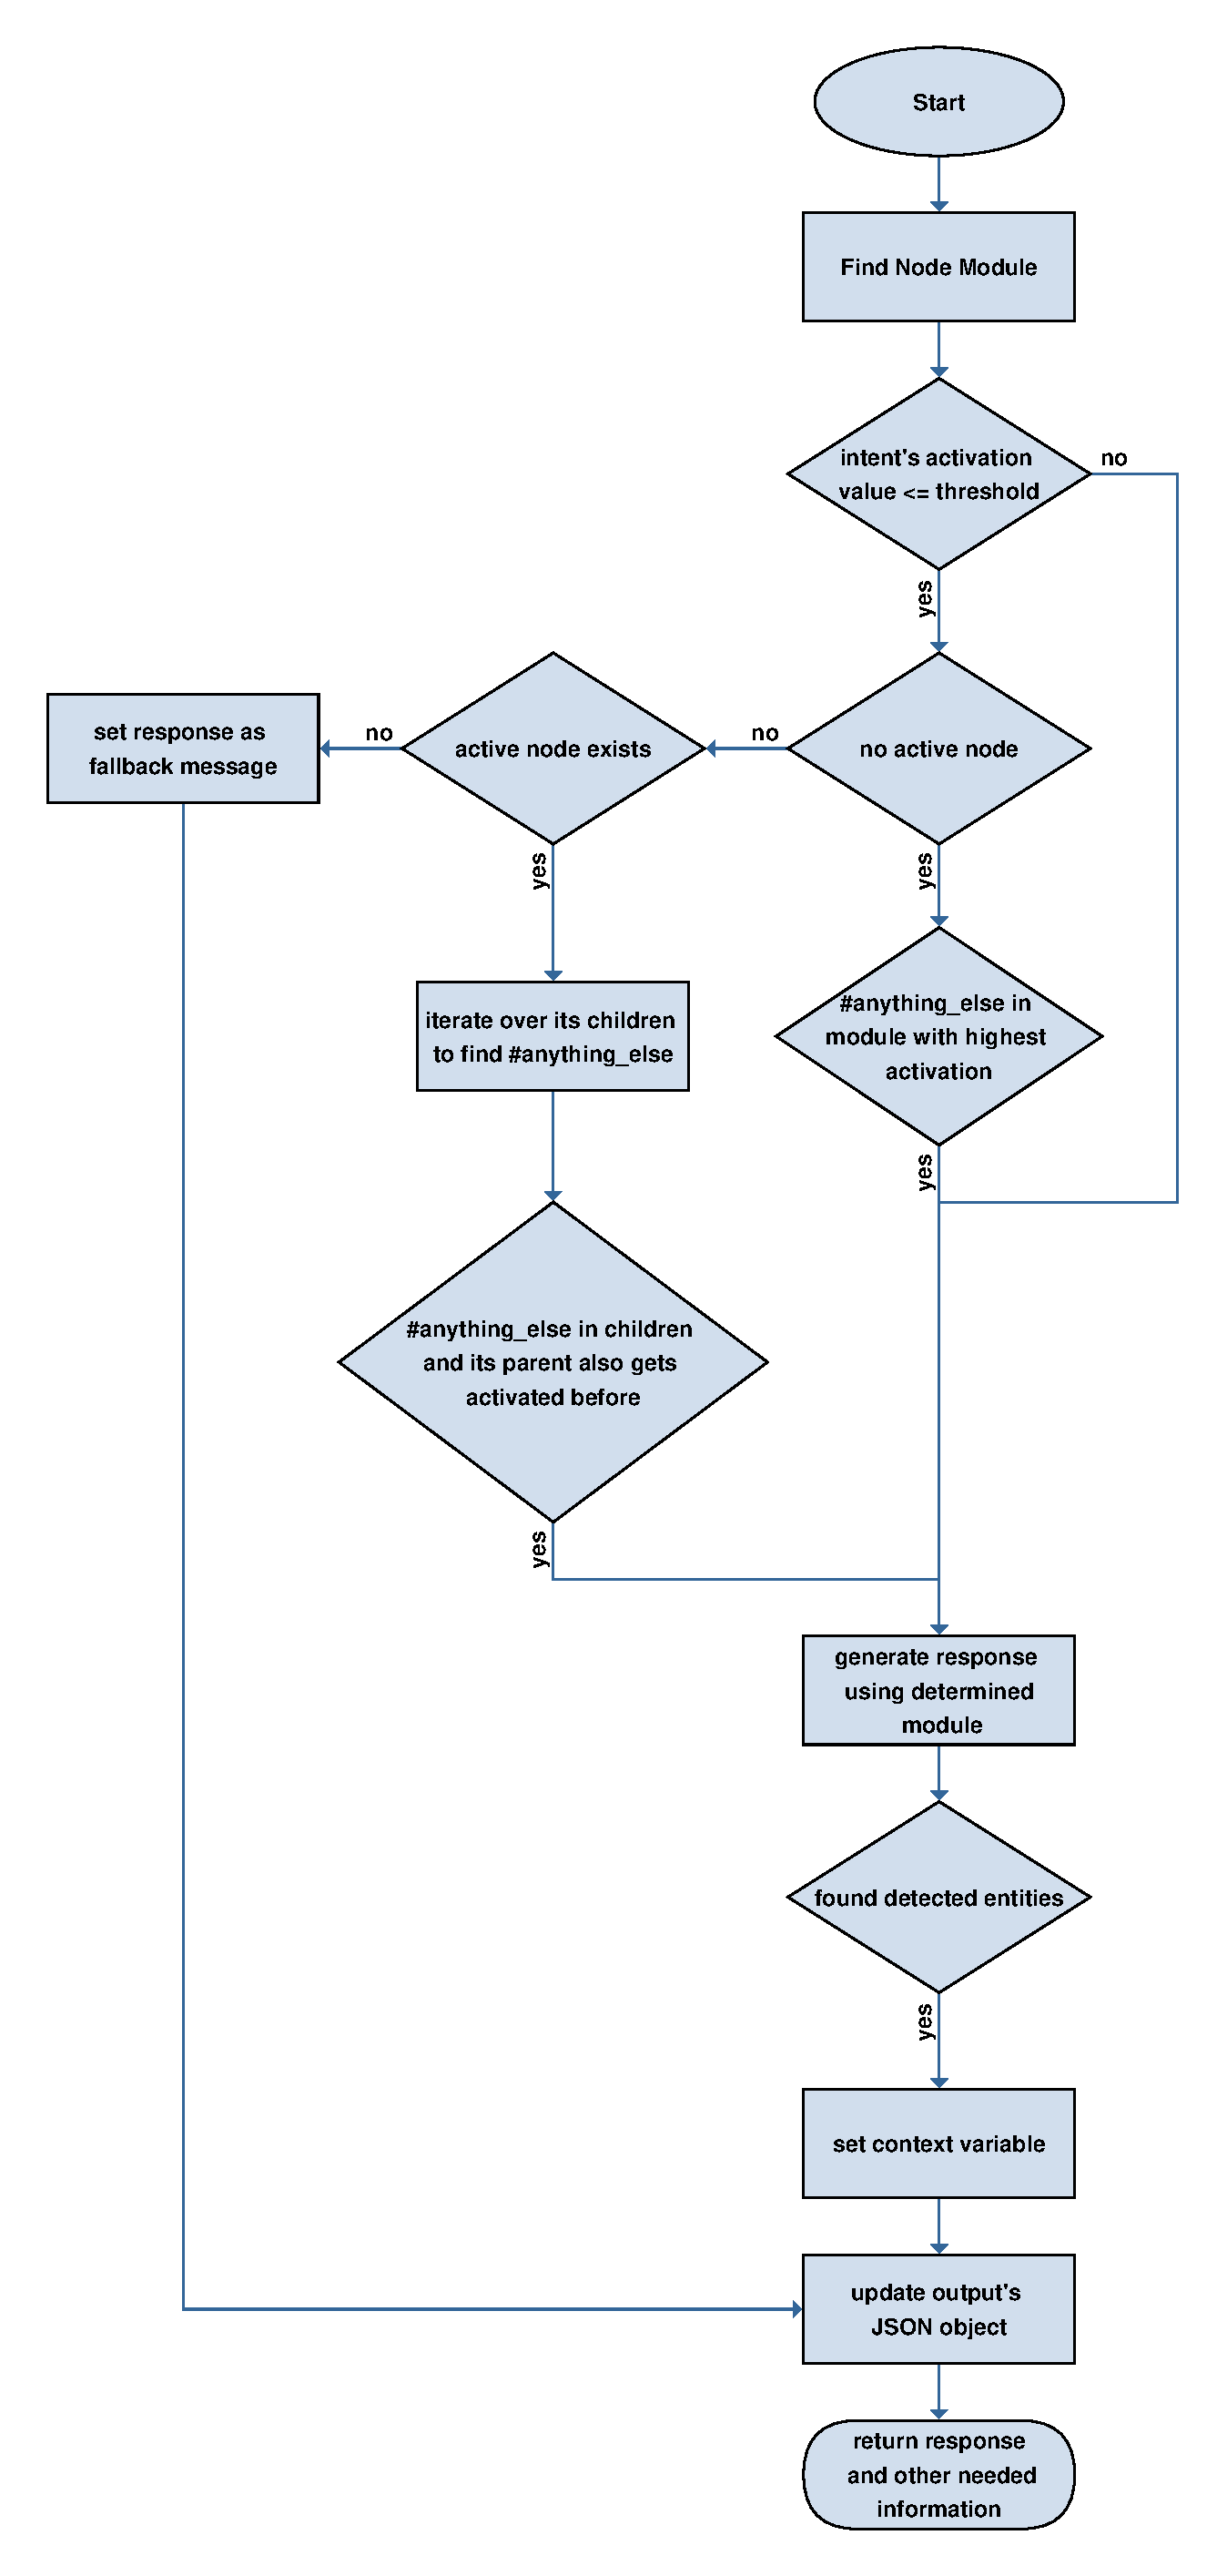
\includegraphics[width=0.6\textwidth]{img/bot.pdf}
    \caption{Flow chart for the bot's say function}
    \label{fig:flowBot}
\end{figure}

\subparagraph*{Dialogue Manager}
Dialogue manager is an abstract class where as max activation dialogue tree manager is an inherited class which should implement the abstract functions of a dialogue manager. Max activation dialogue manager originally contains the dialogue tree, once the chatbot has been initialized. Now the question raises what is the dialogue tree composed of? So, dialogue tree gets generated while chatbot is loaded from the json file. And it is composed of the list of tree nodes, unique module id, data for rasa nlu training and rasa interpreter loaded from model directory once the training has been finished. Whereas, each tree node contains unique node id, information about its parent node,  intent, activation flag which gets set if it is responsible for generating a response and a module object which itself has been consisted of intent detector and response generator. The dialogue tree has been generated using python library "any tree" \cite{anytree}.
\\~\\
It is responsible for finding module with highest activation based upon the detected intent's activation value for the user utterance. So for this purpose each tree must be traversed for each of its node. As each node contains a module object which is further utilized for this purpose. Module's activation function is being called by passing user utterance, rasa interpreter for current module, module id for recent module and session data as parameters. And it returns activation value for each intent along with its name, recognized entities along with their activation values and the json object for output. As activation function for all nodes in each tree has been called and mean while dialogue manager keeps on checking for the activation value received for each node's module. And keeps on updating it whenever the last received value is greater than previously stored value. In this way the module with highest activation is detected.
\\~\\
Responsibility of a dialogue manager not only ends here but it is also responsible to make the chatbot to follow the modular architecture which is a main goal behind the designing of the Frankentbot. As explained above about the modular architecture that how should it work, lets discuss it here in technical perspective. Whenever, the recently received activation value is greater than the last stored activation value and the identified intent is same as the current node's intent name then there comes following scenarios, if the recently traversed node is a root node or not: 
\begin{enumerate}
    \item If it is a root node then its activation flag should be set so that for the next time its children can be accessed for response generation. Also, all the required information must be stored and returned to the previously discussed bot component. Which is responsible for returning the response to the client via web API and the active state for the current user must get updated beforehand. 
    \item Secondly, if recently processed node is not a root node then what should be its behaviour? Its a bit complex strategy to follow. Firstly, it should check if its parent's activation flag is set or not. If it is set then it should proceed further otherwise it should not. Lets suppose that it is set and it steps ahead and finds multiple nodes with same intent in its children nodes then it will not respond correctly. As, it is the main idea behind modular architecture that modules can be reused but it is not necessary that module with the same intent have same response. Responses can differ at different levels in a tree whilst having same intent. So for removing this problem, active state for each module has been stored separately. Which means if there exist two modules for a chatbot then there should be two separate active states, one for each module, available for a user. So by using these active states, it can match the last active node's id with current node's parent id and if it is true then it is good to go. Also what if user starts to enter the same user utterance again and again. It will again cause a problem as it will be searching for an intent in last active node's children but it will not be able to find it. So to overcome this issue, manager matches the current node's id with last active node's id and again if this condition has been satisfied then it should respond correctly. 
    \item Lastly, irrespective of the above conditions whether any of them is satisfied or not. It should return to a bot component which is meant to handle all scenarios and responsible to produce an appropriate response if there exists any highest detected module. Otherwise, it uses anything\_else node or fallback message to respond depending upon the state and design of the bot.
\end{enumerate} 
\\~\\
At the end, it also checks for identified entities and their activation values and stores and updates them accordingly. And all the essential information is returned to a bot component. Which is responsible for returning the response to the client via web API and the active state for the current user should be updated beforehand. Detailed visual chart for it is portrayed below in the Figure \ref{fig:flowDialogueMan}.

\begin{figure}[!h]
    \centering
    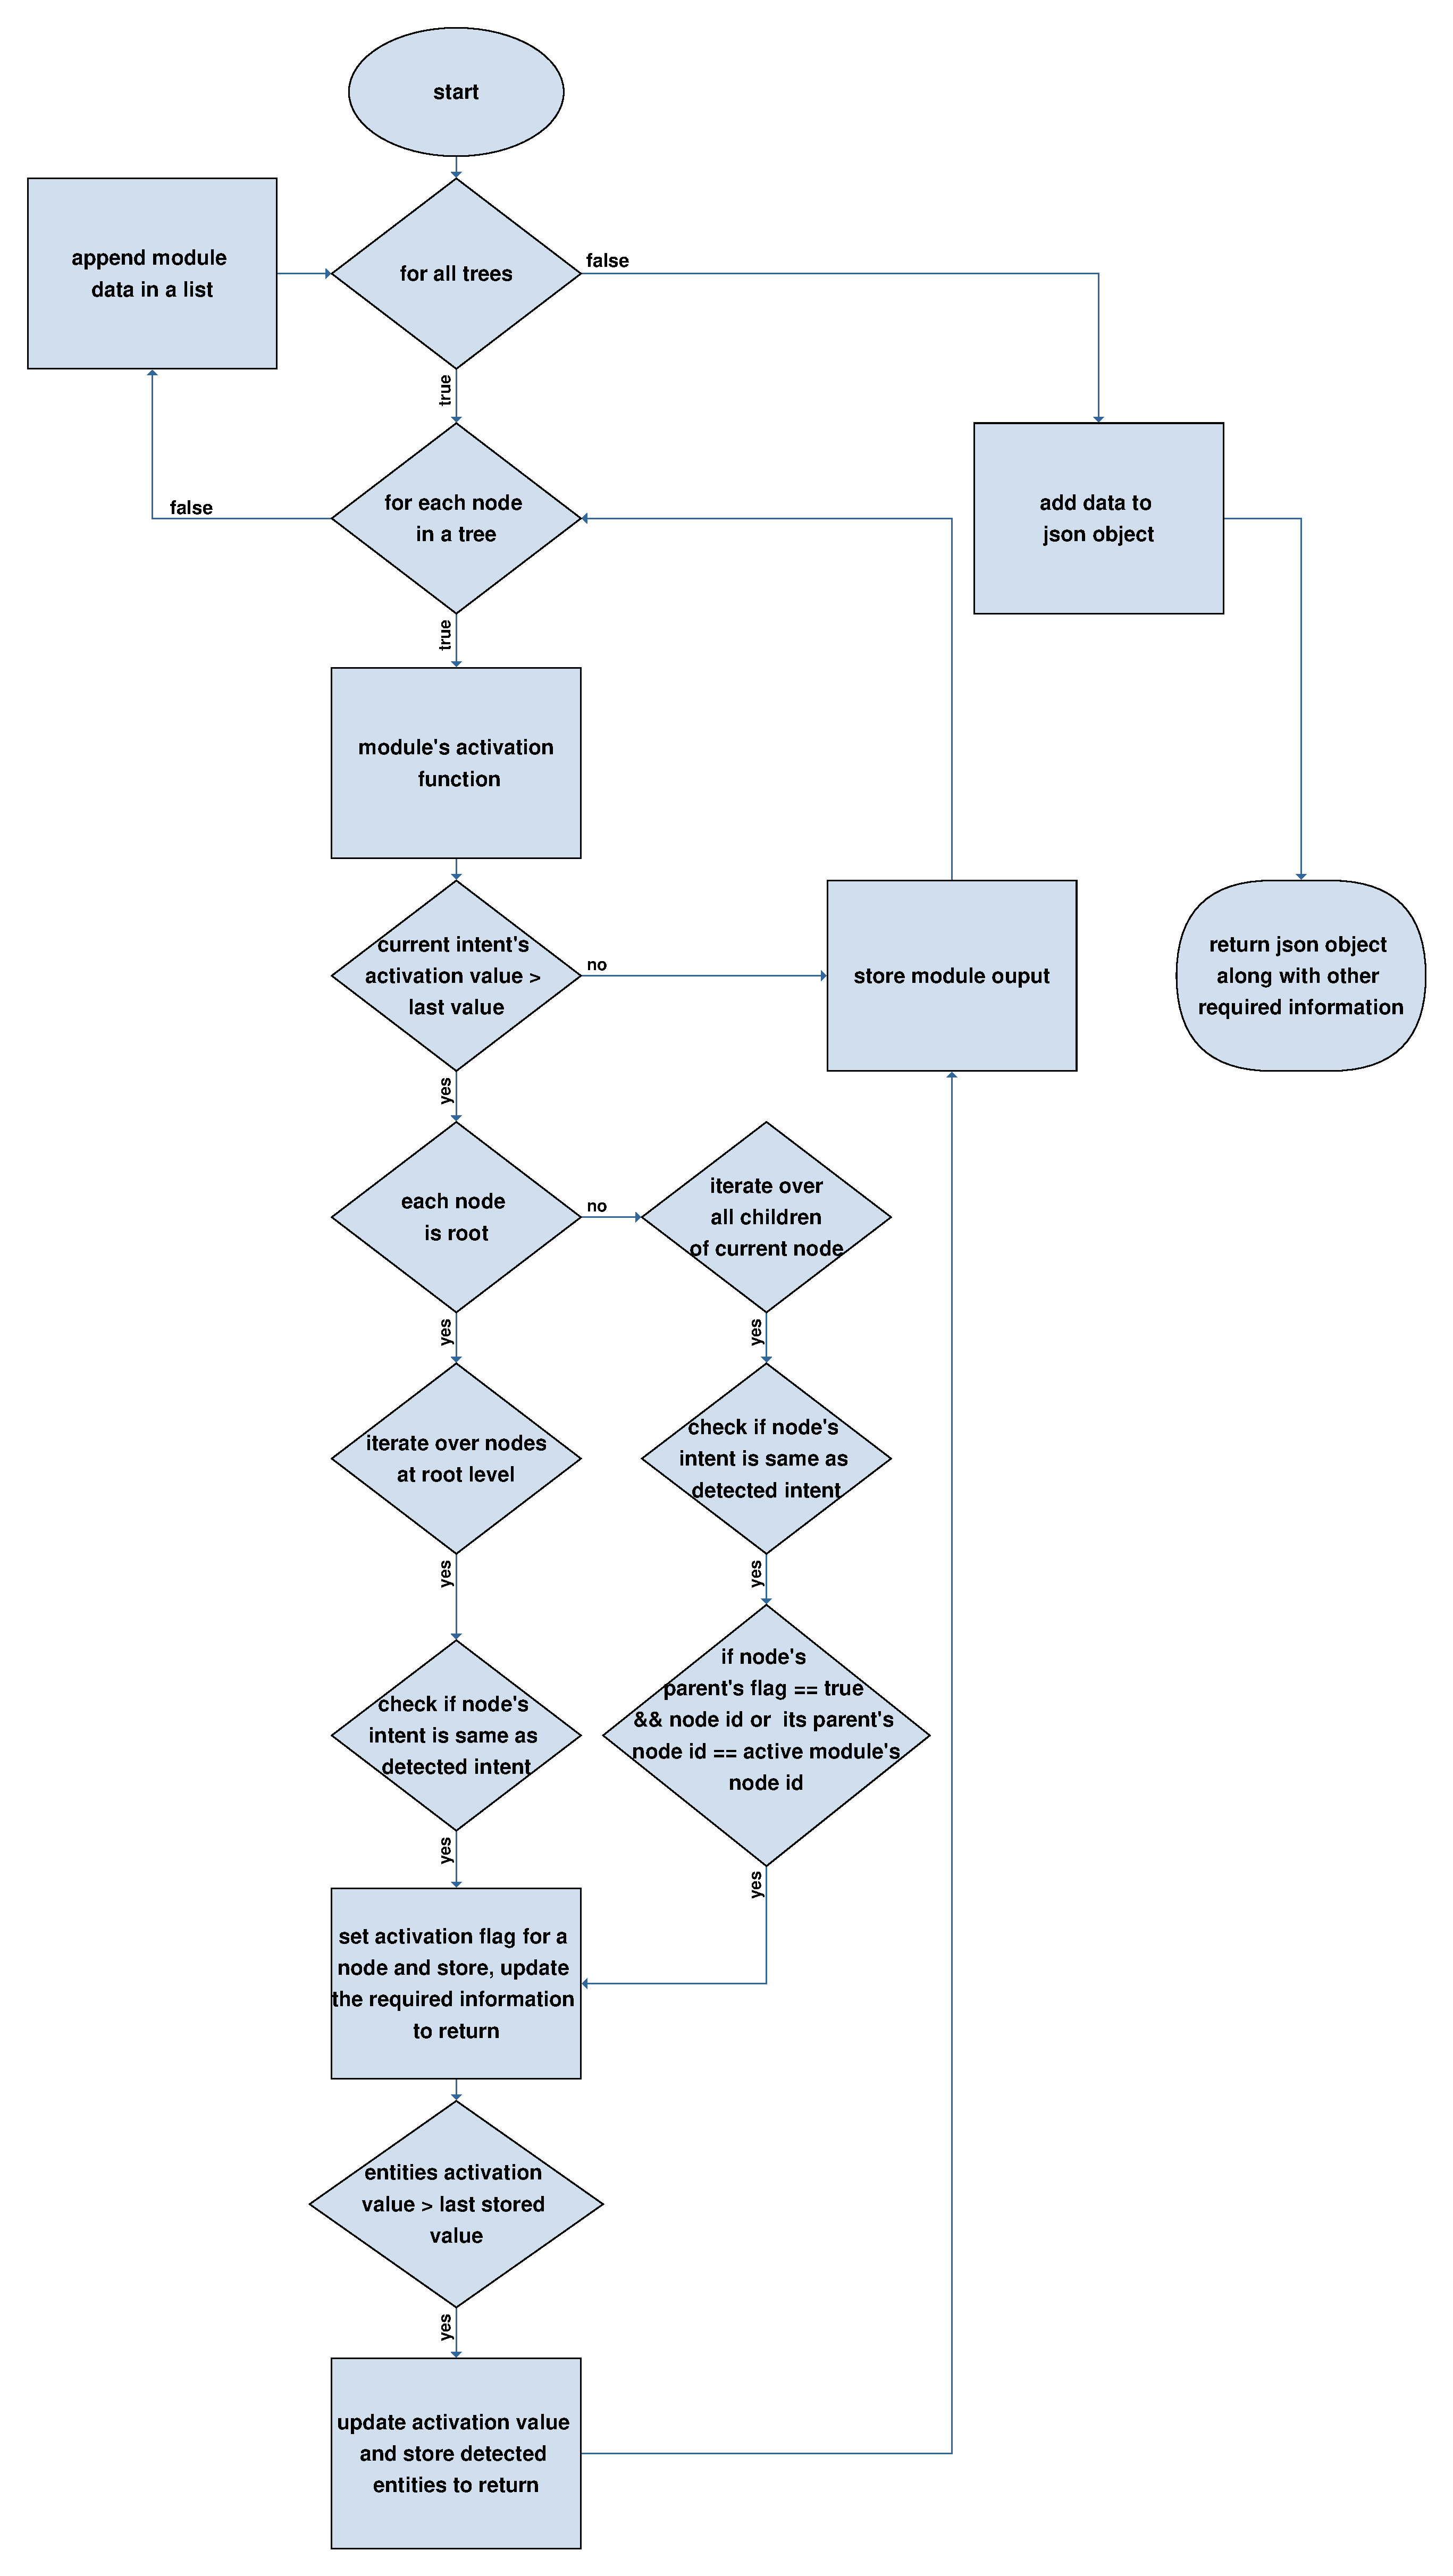
\includegraphics[width=0.7\textwidth]{img/Dialogue_manager.pdf}
    \caption{Flow chart for the dialogue manager's find node module function}
    \label{fig:flowDialogueMan}
\end{figure}

\subparagraph*{Modules} Modules class is responsible for generating activation value for each intent which is passed to dialogue manager for further processing as described above. In addition to that, it is also pledged for generating response and json object for API output. So these three functionalities should be implemented in a class inherited from abstract modules class. So, class Atom is inherited from it and provides all functional definitions for abstract class. 
\\~\\
There are two attributes needed for atom class. One is natural language understanding(nlu) which is an object for rasa intent and entity detector and second is a simple response generator's object, Both of these components has been described next under their respective headings. 
\\~\\
Starting with an activation function, from a max activation dialogue manager's function to find a node's module with highest activation value, all trees are traversed for each corresponding node. Each node contains particular module object with its own nlu and response generator. Using that module, activation function has been called provided user utterance, rasa interpreter, recent module id for a tree and session information as parameters to it. And what it does with these parameters received is, it passes them further to make a call for natural language understanding to detect intents and entities. And the encountered intents and entities are then further passed for creating json object to return to the client as api output. Graphical representation for it can be visualized in the Figure \ref{fig:flowModule}.

\begin{figure}[!h]
    \centering
    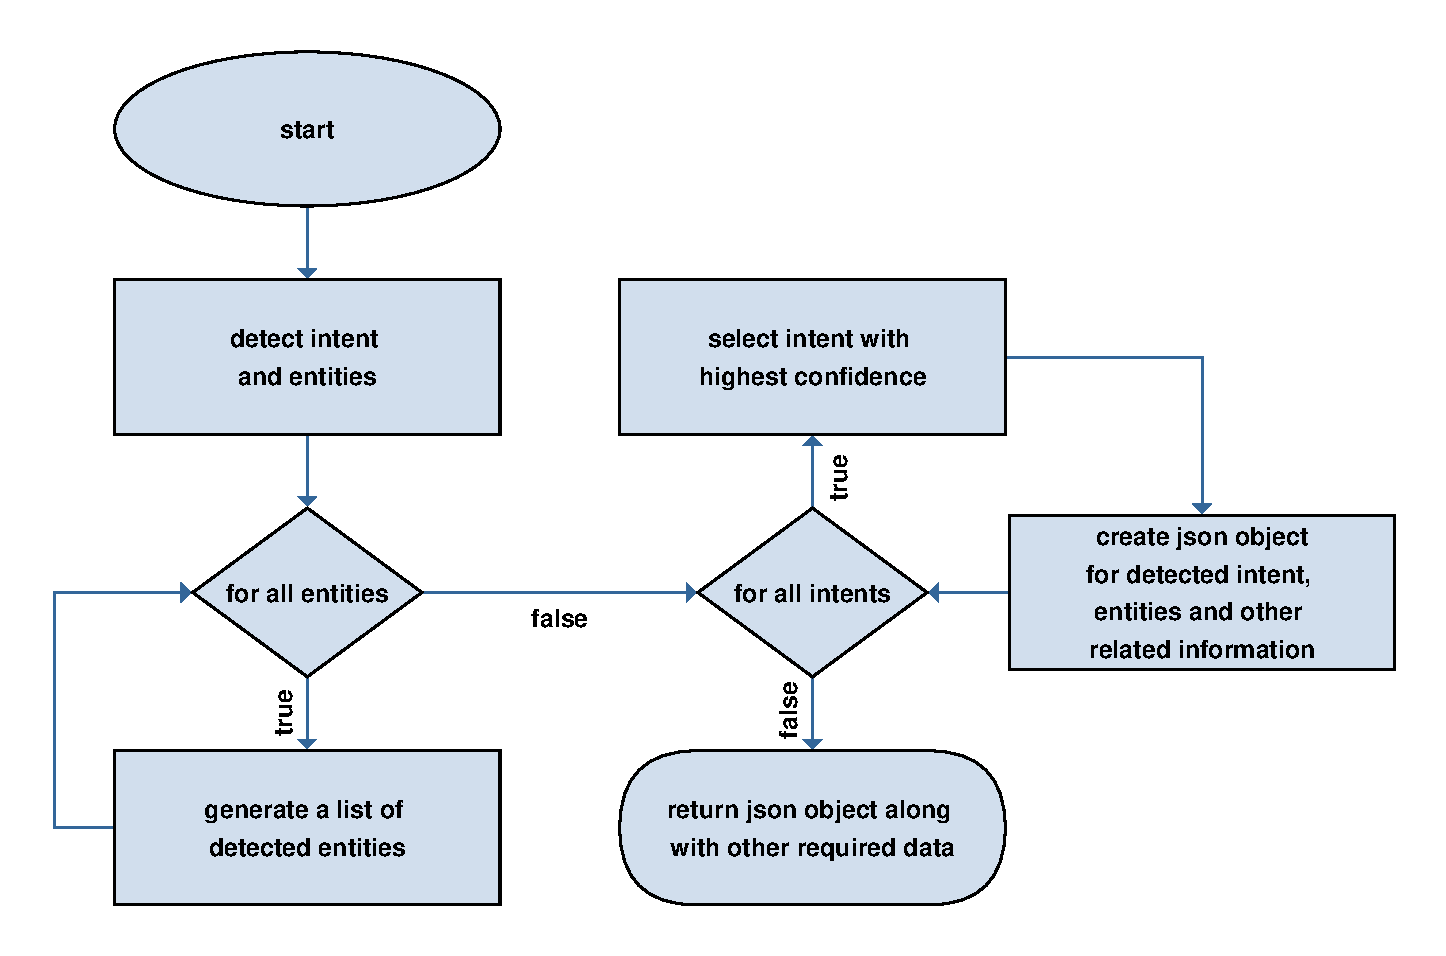
\includegraphics[width=0.9\textwidth]{img/module.pdf}
    \caption{Flow chart for the module's activation function}
    \label{fig:flowModule}
\end{figure}
\\~\\
Moreover, it also has been used to generate a response with the help of response generator for an encountered module with a highest activation based upon the identified intent and entities for a particular user.

\subparagraph*{Intent and Entity Detection}
It is the one of the basic and necessary components for all chatbots. Same applies to Frankenbot. Intent and entity detector is responsible for identification of an intent and entities for an user utterance. So this feature must be handled within a successor class for it. So rasa intent entity detector is implementing this functionality for an abstract parent class.
\\~\\
Each tree node consists of an atom and each atom consists of the intent and entity detector with the intent and entities information stored for each node. It is responsible to detect the intent and all the entities for the user utterance by utilizing the parametric rasa interpreter passed to it from atomic activation function.
\\~\\
Coming towards internal processing, the user utterance is passed to the trained rasa interpreter in order to detect the intent and entities and matched with the current node's intent. If they have been appeared to be identical then the intent name is stored as a key in a dictionary object and a confidence value received from the result of rasa interpreter represents its value. Also, the entities are stored as a list of dictionary objects and each object contains key value pairs for entity name and confidence value, starting and ending index in an utterance. These detected intent and entities are returned from this function to its origin for further handling. Visuals have been displayed in the Figure \ref{fig:flowIntandEnt} exhibiting comprehended process.

\begin{figure}[!h]
    \centering
    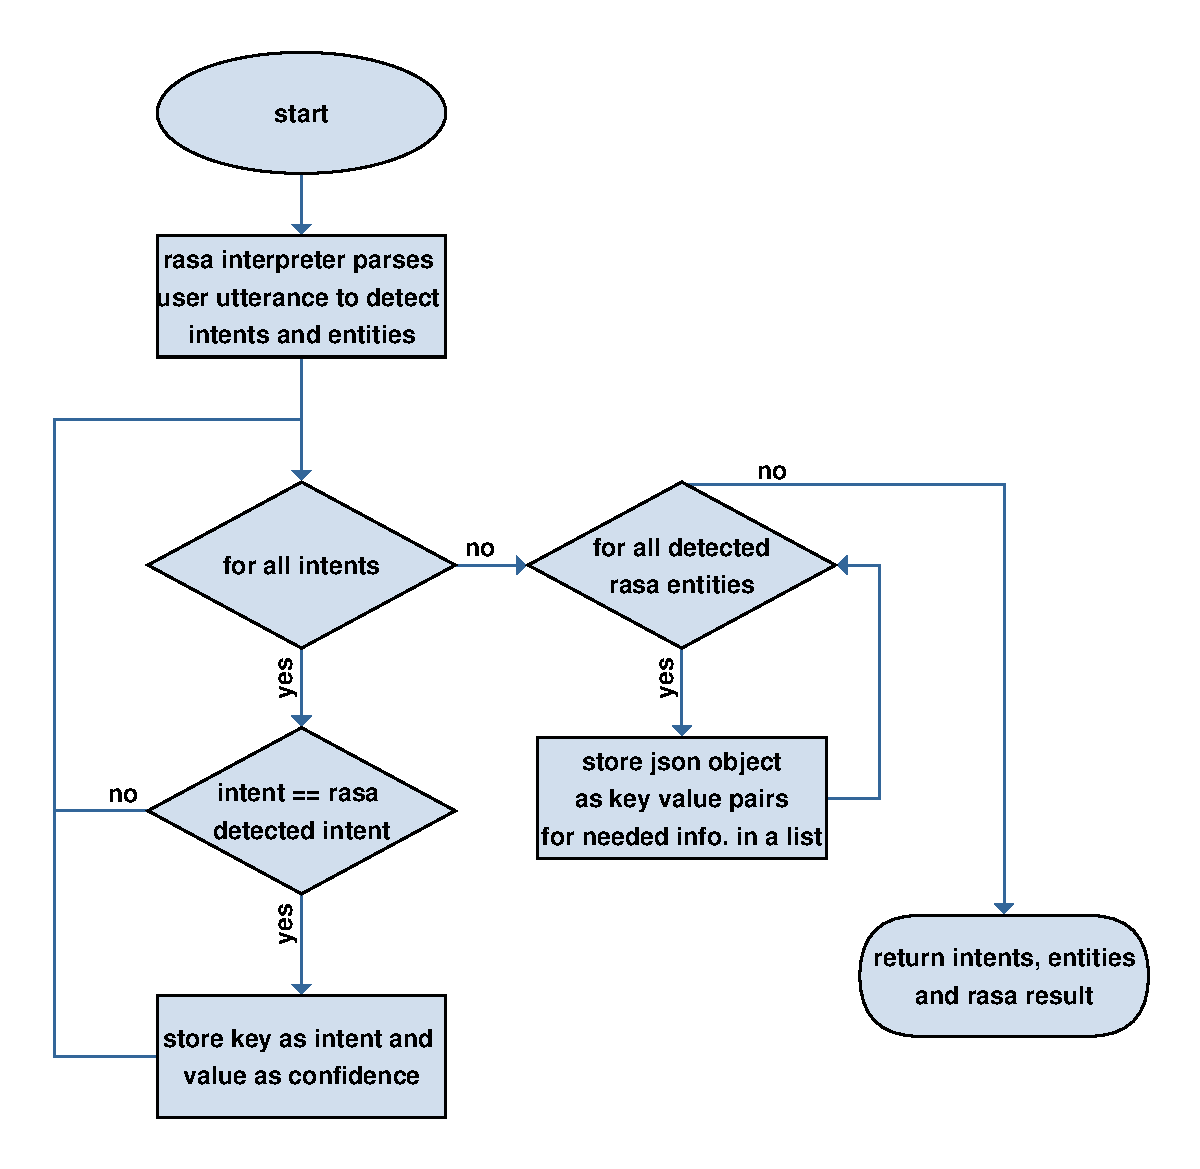
\includegraphics[width=0.9\textwidth]{img/Intent_entity_detector.pdf}
    \caption{Flow chart for the Rasa Intent and Entity Detector}
    \label{fig:flowIntandEnt}
\end{figure}

\subparagraph*{Response Generation}
Response generation is an ultimate goal for any chatbot. As the name itself is much self explanatory that what task should it perform. Response generator is liable for producing a response taking in to account an identified intent. Additionally, it is also responsible for appending chatbot response to the final json object designed to be returned as an api output. 
\\~\\
It is compulsory for the precedent classes to take in to account both of the functionalities that parent abstract class is responsible for. Simple response generator does it all for Frankenbot. As it needs mode for a response that can be sequential or random and a list of responses for a captured intent for response selection.
\\~\\
Once the pre-processing has been completed, means all the steps have been finished and dialogue manager has returned the atomic module with highest activation value and a chatbot needs to generate a response. Now, a bot uses that observed module to send request to this component by providing it with recognized intents and entities along with session information as an input. So that it can go ahead and perform the task that it is responsible for. 
\\~\\
Firstly, it will check for the intent's sequential response counter for a specific user and updates it accordingly for the next time usage. Secondly, after selection of a response, it checks within a response for entities and context variables. If there is any detected entity for a user utterance and a response needs to be exchanged with its value then it should be handled here. Also, if there is any context variable stored previously for a user and bot's reply needs to get modified with its value then it should also be done here. After all processing has been accomplished, it should create a json object with a chatbot response for api output and send it back to a bot component for performing next required executions. Its graphical representation is shown in the Figure \ref{fig:flowRespGen} below. 

\begin{figure}[!h]
    \centering
    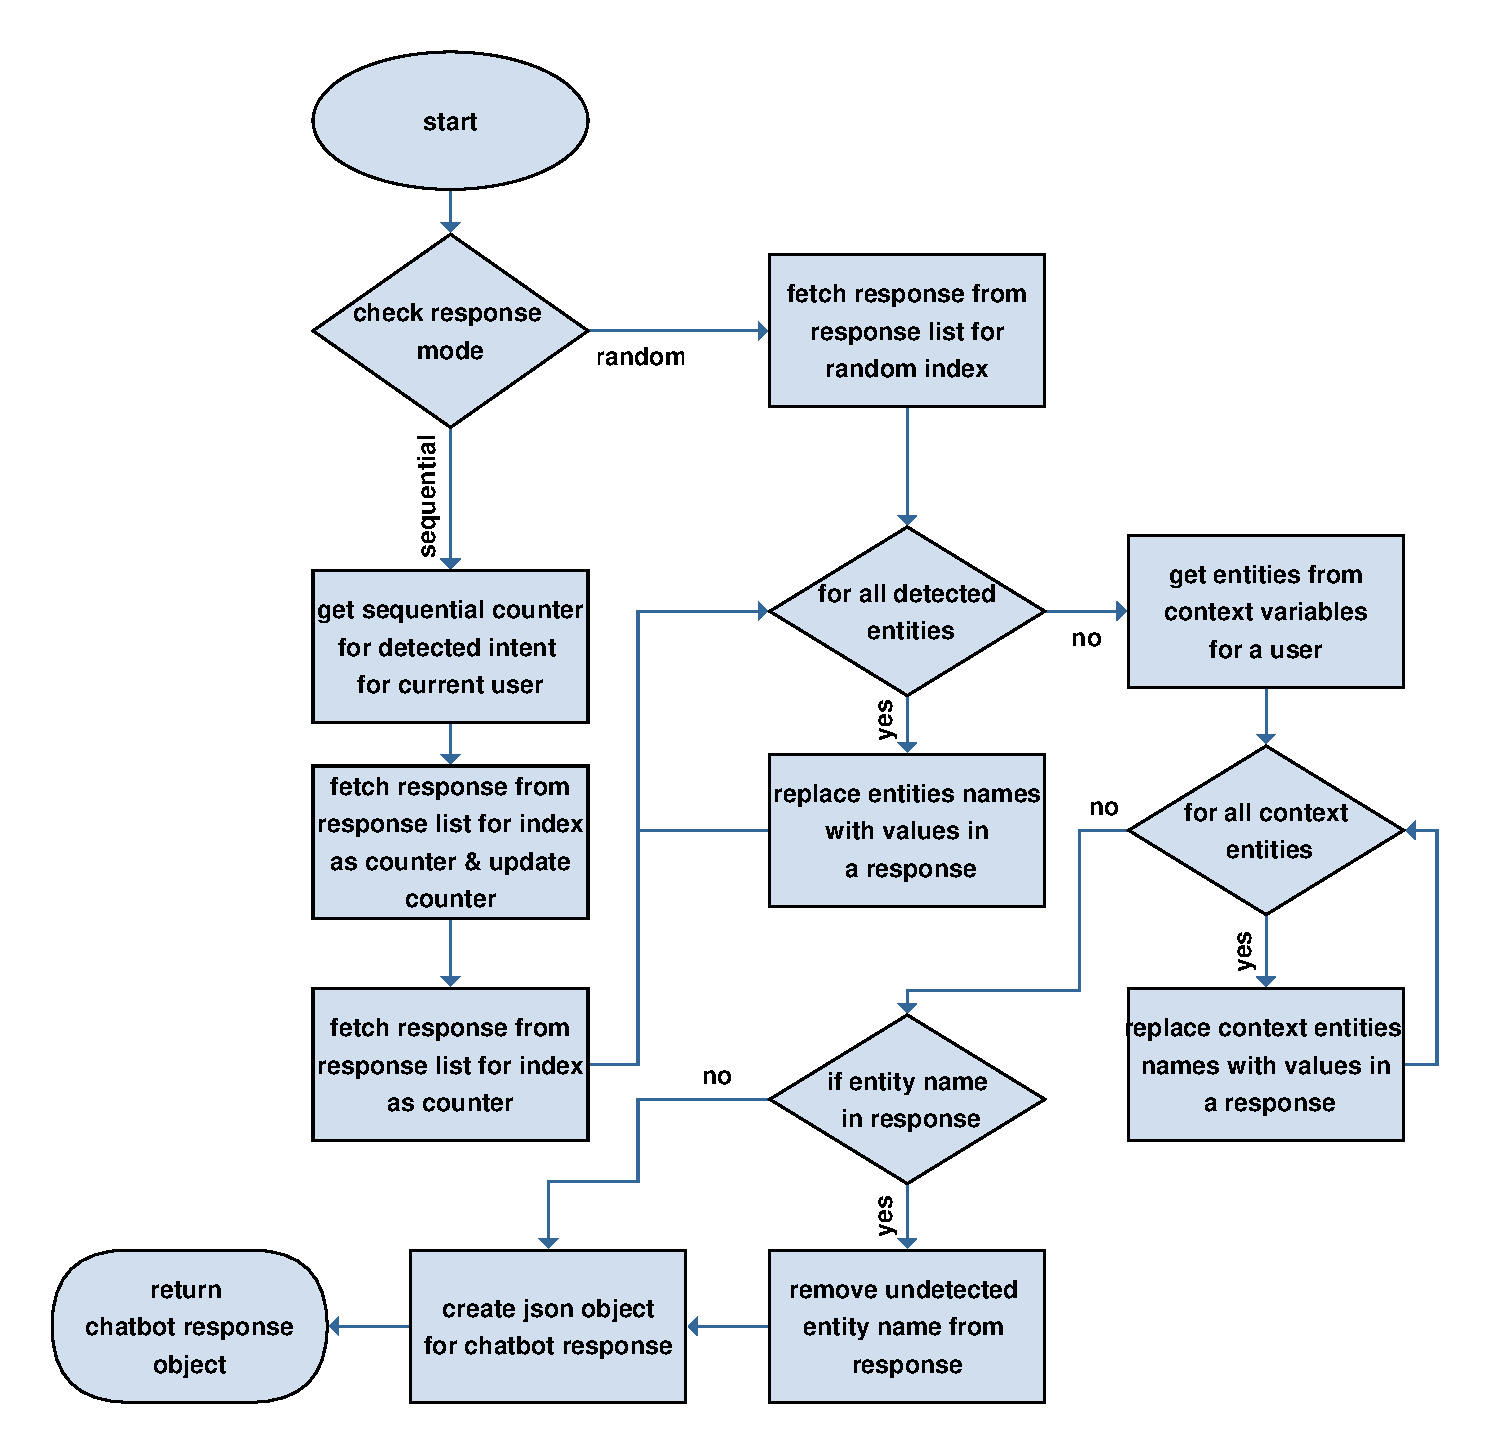
\includegraphics[width=0.9\textwidth]{img/Response_generator.pdf}
    \caption{Flow chart to generate response }
    \label{fig:flowRespGen}
\end{figure}

\subparagraph*{JSON API Output}
After all components are done with their part, bot returns a json object to web api and api returns it further to a client which is parsed at client side for displaying needed information for a user. Lets start with a observation of json object demonstrated below:

\begin{lstlisting}[language=json, firstnumber=1]
{
    "user_utterance": {
        "text": "..."
    }, 
     "chatbot_utterance": {
        "type": "simple_response", 
        "response": "..."
    },
    "active_module": {
        "id": "...", 
        "type": "dialog_tree_module", 
        "activation_value": ..., 
        "module_output": {
            "recognized_intent": "...", 
            "recognized_entities": []
        }
    }, 
    "modules_output": [
        {
         "id": "...",
         "type": "dialog_tree_module",
         "activation_value": ... ,
         "module_output": {
            "recognized_intent": "...",
            "recognized_entities": [],
            "intent_ranking": [
               {
                  "name": "...",
                  "confidence": ...
               },
               ... ,
            ]
         }
      },
      ... ,
    ]
}
\end{lstlisting}
The json object contains user\_utterance which holds a key text for user's message as a value. Secondly, chatbot\_utterance's response is a final reply of a chatbot. An active\_module reflects an id of recognized module, activation\_value in terms of rasa's confidence value for an identified intent. Whereas, its child module\_output depicts an encountered intent and detected entities. Finally, modules\_output involves the dictionary object for all modules in a chatbot through which user utterance has been processed in order to generate a response after intent detection. So, id shows an id of a module, activation\_value is same just like as mentioned before for active\_module. Furthermore, module\_output is also similar to active\_module's module\_output but with an additional key for intent\_ranking. It is comprised of all the names for the intents and their respective confidence values obtained from rasa's trained natural language interpreter.

\subparagraph*{Logging}
It is something that has been used commonly now a days to track the events occurring in any software or a system. 
\\~\\
For the framework, it has been implemented using python's library called "logging" \cite{logging}. Before returning the JSON object via web API to the client, this object with all the essential information from start i.e. received user utterance, till end i.e. generated suitable response, has been logged to a log file in order to keep track of the complete dialogue. Also, log file contains the information for rasa's nlu training process and what intents and entities have been found in training data. Additionally, it also helps in tracking the error or reason of the chatbot failure, if any such event occurs.  


